\documentclass{article} 
% \usepackage{iclr2026_conference,times}
\usepackage{macros}
\usepackage{hyperref}
\usepackage{url}
\usepackage[toc,page,header]{appendix}
\usepackage{geometry}
\geometry{margin=1in}

\usepackage{minitoc}

\renewcommand \thepart{}
\renewcommand \partname{}

\title{A Unifying Framework for Concept-Based Representational Similarity}

\author{}

\newcommand{\greg}[1]{{\color{indigo}[Gregoire]: #1}}
\newcommand{\fel}[1]{{\color{gold}[Fel]: #1}}
\newcommand{\agus}[1]{{\color{green}[Agus]: #1}}
\newcommand{\boutin}[1]{{\color{pink}[Baltringueur]: #1}}


\begin{document}

\doparttoc % Tell to minitoc to generate a toc for the parts
\faketableofcontents % Run a fake tableofcontents command for the partocs

\maketitle

\begin{abstract}
...
\end{abstract}

\begin{figure}[h]
    \centering
    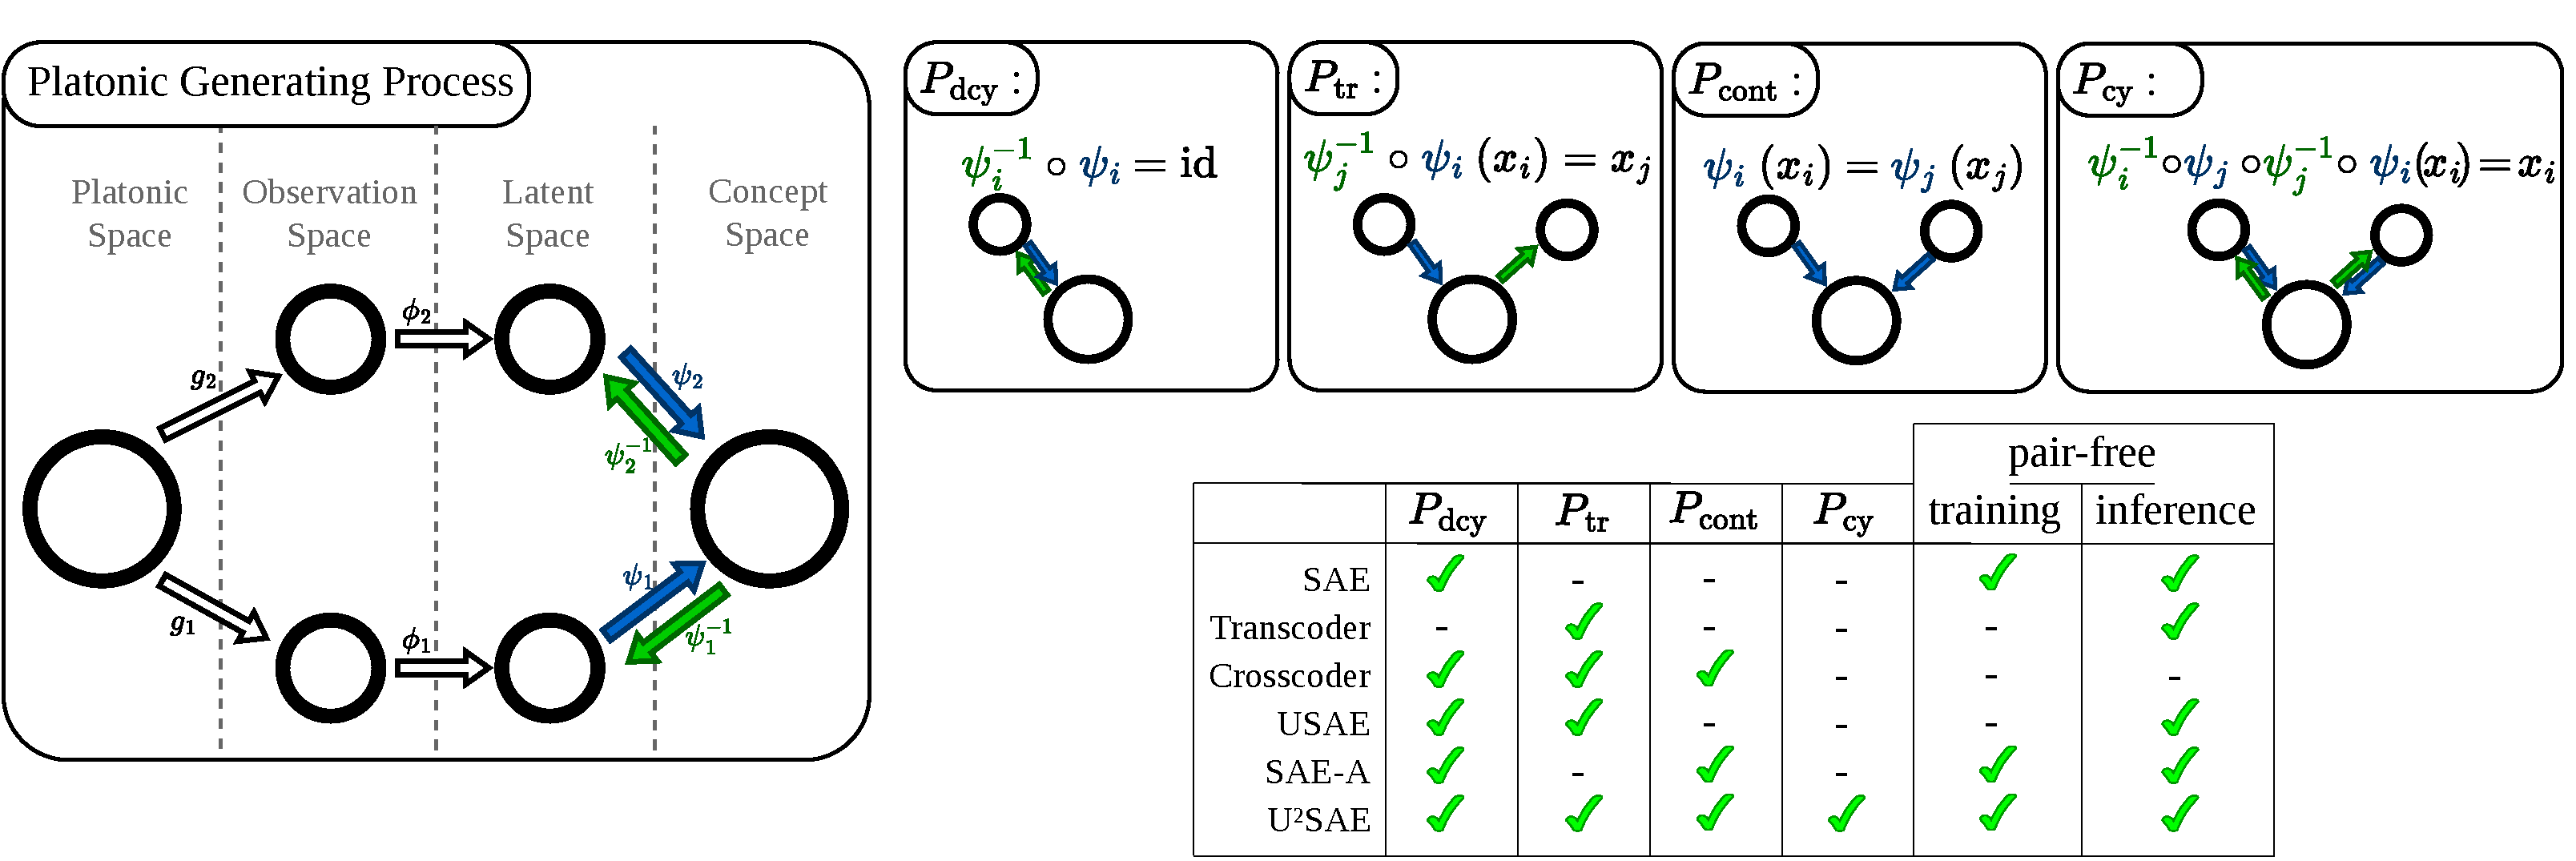
\includegraphics[width=0.99\textwidth]{figures/CoSAE_banner_v0.pdf}
    \caption{Summary of the proposed framework. \textbf{Left :} Illustration of the platonic representation hypothesis through a generative process. Observation stem from a shared space through modality specific generators $g_i$. Feature extractors ($\phi_i$) learn to invert this generative process up to some transform $\psi_i$. \textbf{Top~right~:} Different properties that can be enforced on $\psi_i$ to achieve different types of alignment. \textbf{Bottom~right~:} summary of previous SAE-based methods for concept extraction along with which property they are trained to satisfy.\greg{TODO: enlarge function symbols in the DGP part}}
    \label{fig:framework}
\end{figure}

\section{Introduction}

\section{Related work}

interpretability history : feature vis, attribution, then circuit discovery and concept decomposition (NMF, ICA, SAE).

representation alignment - coarse grained, global summary of linear structure

crosscoders, USAE, SAE-A - fine grained, concept level description of shared structure

\greg{https://x.com/mariabrbic/status/2023767525285151154?s=20 : representation alignment = shit -> motivate even more concept alignment ?}

\greg{Revisiting the Platonic Representation Hypothesis: An Aristotelian View}

\section{Framework formulation}

\paragraph{Concept Alignment.} Let $I$ be an index set whose elements correspond to representation instances. Each $i \in I$ may, for example, index the same modality embedded in different models, different layers of a single model, checkpoints of a single model at different training steps, modality specific instantiations of an abstract idea, etc. Let $X$ be a set of data points equipped with a measure $\mu$, and $\phi_i : X \to \R^d$ be a representation function for each $i \in I$. Denote by $X^i \coloneq \phi_i(X)$ the set of representations of $X$ under $\phi_i$, and by $\mu_i \coloneq \phi_i \# \mu$ the pushforward measure on $X^i$ induced by $\phi_i$. Let $\psi_i : X^i \to \R^K$ be concept extraction functions with corresponding decoders $\psi_i^{-1} : \R^K \to X^i$ suspiciously denoted with the inverse notation.
%
Under this setting, we can define the following alignment properties of \emph{translation} and \emph{concept consistency} at the instance level~:
%
\noindent
\begin{minipage}{0.49\textwidth}
\begin{align}
\label{eq:pair_wise_properties}
\Ptr: \quad & \forall i, j \in I, \forall x \in X, \quad (\psi^{-1}_j \circ \psi_i) (x_i) = x_j \\
\Pcont: \quad & \forall i, j \in I, \forall x \in X, \quad \psi_i(x_i) = \psi_j(x_j)
\end{align}
\end{minipage}
\hfill
\begin{minipage}{0.49\textwidth}
\vspace{2mm}
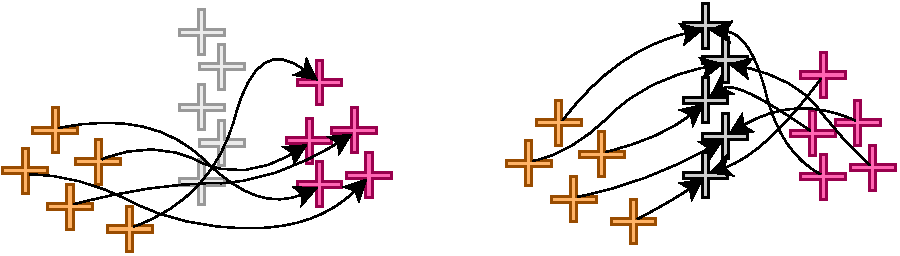
\includegraphics[width=\linewidth]{figures/tr_cont_illustration.pdf}
\captionof{figure}{Illustration of $\Ptr$ (\emph{left}) and $\Pcont$ (\emph{right}) properties with pair-wise correspondences.}
\vspace{2mm}
\end{minipage}
%
Where $x_i = \phi_i(x)$ and $x_j = \phi_j(x)$. If the $X^i$ are such that instance wise correspondences are not available, i.e. we do not have acces to the underlying $X$, we can translate these into distribution wise alignment properties as follows:
%

\noindent
\begin{minipage}{0.49\textwidth}
\begin{align}
\label{eq:distribution_wise_properties}
\Ptrdist: \quad & \forall i, j \in I, (\psi^{-1}_j \circ \psi_i) \# \mu_i = \mu_j \\
\Pcontdist: \quad & \forall i, j \in I, \psi_i \# \mu_i = \psi_j \# \mu_j
\end{align}
\end{minipage}
\hfill
\begin{minipage}{0.49\textwidth}
\vspace{2mm}
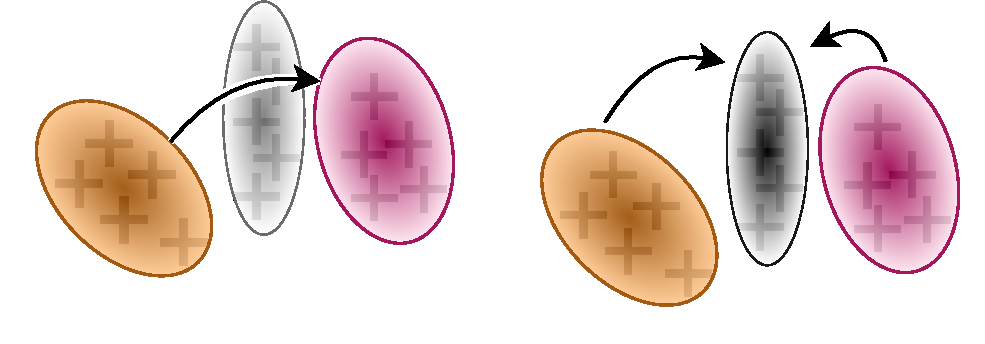
\includegraphics[width=\linewidth]{figures/tr_cont_dist_illustration.pdf}
\captionof{figure}{Illustration of $\Ptrdist$ (\emph{left}) and $\Pcontdist$ (\emph{right}) properties free of pair-wise correspondences.}
\vspace{2mm}
\end{minipage}
%
where $(\psi^{-1}_j \circ \psi_i) \# \mu_i$ defines a measure on $X^j$, and $\psi_i \# \mu_i$ defines a measure on the concept space $\R^K$. In addition to these alignment properties, we can also define standard autoencoding properties, effectively stating that $\psi^{-1}_i$ is indeed the inverse of $\psi_i$ on the support of $\mu_i$~:

\noindent
\begin{minipage}{0.54\textwidth}
\begin{align}
\label{eq:dcy}
\Pdcy: \quad & \forall i \in I, \forall x_i \in X^i, \quad (\psi^{-1}_i \circ \psi_i) (x_i) = x_i \\
\Pcy: \quad & \forall i, j\!\in\!I, \forall x_i\!\in\!X^i, (\psi^{-1}_i\!\circ\!\psi_j\!\circ\!\psi_j^{-1}\!\circ\!\psi_i) (x_i) = x_i
\end{align}
\end{minipage}
\hfill
\begin{minipage}{0.45\textwidth}
\vspace{2mm}
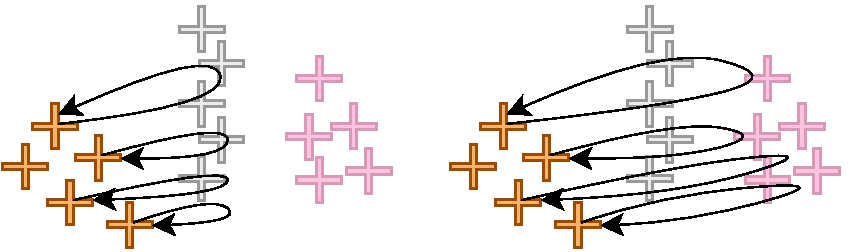
\includegraphics[width=\linewidth]{figures/dcy_cy_illustration.pdf}
\captionof{figure}{Illustration of $\Pdcy$ (\emph{left}) and $\Pcy$ (\emph{right}) properties.}
\vspace{2mm}
\end{minipage}
%
The \emph{demi-cycle} property $\Pdcy$ is the standard reconstruction objective of autoencoders, while the full \emph{cycle} $\Pcy$ is an alternative way to align autoencoders without requiring instance wise correspondences through reconstruction only.

\paragraph{Alignment Dualities.} As shown by \citet{TODO:rufin}, there is a duality between $\Ptr$ and $\Pcont$~: asssuming both $\Pdcy$ and that the $\psi^{-1}_i$ are injective on the support of the shared concept space, we have that~:
%
\begin{align}
\label{eq:duality}
\Ptr \iff \Pcont
\end{align}
%
We show in \cref{sec:translation_vs_concept_consistency} that this duality does not even hold in synthetic settings with controlled data generating processes.
%
This is not the only duality at play, as instance-wise $\Ptr$ (resp. $\Pcont$) also implies distribution-wise $\Ptrdist$ (resp. $\Pcontdist$) without any additional assumption. However, the converse does not hold in general, and requires additional assumptions on the distributions and the class of functions under consideration. These strong assumptions are unrealistic in practice (see \cref{sec:instance_vs_distribution_alignment}). We show in \cref{sec:anchoring} that this duality can be restored, gaining the converse implication using only a small set of anchor points with known correspondences. Finally, \citet{TODO} show empirically that in natural language processing (NLP) for translation settings, $\Pcy$ is enough for pair-free training of translators, i.e. without instance wise correspondences. We discuss this in \cref{sec:cycle_consistency}.

Recent works for joint concept recovery focuses only on subsets of these properties with little to no discussion on the other ones, and of their interactions. This motivates the need for a unifying framework to understand the properties and assumptions underlying the different methods used in the literature, and to design new methods that can better enforce these properties for future concept alignment studies.

\paragraph{Platonic Representation Hypothesis (PRH).} The PRH is a universal statement that any representation learning method will converge to the same shared representation, up to some transform \citep{TODO}. This can be formalised in various ways. We chose to write this hypothesis in under a generative framework as it allows for a formulation that is ready to be plugged into our above framework. The generative view of the PRH assumes the existence of a platonic latent space $X$ such that all real world observations, whatever their domain $\mathcal{X}^i$, stem from this platonic latent space through a generator $g_i : X \to \mathcal{X}^i$. Then, all feature extractors $\phi_i : \mathcal{X}^i \to X^i$ invert this generative process up to a transform $\psi_i$. In the context laid out above, adding this extra generative step allows for intermediate observation spaces $(\mathcal{X}^i)_{i \in I}$ between the platonic latent space $X$ and the feature extractors $\phi_i$. This is especially relevant when the $g_i$s are allowed to introduce distribution shifts or even modality shifts. For simplicity, we can further add the restriction that $X = \R^K$.

\begin{hypothesis}[Platonic Generative Process]
\label{hyp:generative_process}
$\exists K\!\in\!\N, \exists X\!\subseteq\!\mathbb{R}^{\K}$ s.t. $\forall i\!\in\!I$
%
\begin{align}
    &\exists g_i:X\!\to\!\mathcal{X}^i\\
    &\forall \phi_i:\mathcal{X}^i\!\to\!X^i, \exists \psi_i:X^i\!\to\!X,\text{ s.t. }\psi_i\circ\phi_i\circ g_i=\operatorname{id}_{X}
\end{align}
%
\end{hypothesis}

\paragraph{Linear Representation Hypothesis (LRH).} In practice, most of recent representation alignment and concept extraction methods implicitely assume the existence of such a generative process. In other words, they assume that representation learning inverts the generative process. In the case of representation alignment, the class of $\psi_i$ under consideration is further constrained, allowing invariance up to translation, scaling, orthogonal transformations, etc. Dictionary learning based methods fall under a different assumption, more realistic, and grounded in neurosciences : that platonic representations are \emph{sparse} (\Cref{hyp:sparse_inversion}), imposing different constraints on $\psi_i$. This sparse coding framework often comes with additional linear, or close to linear constraints. The reason is (\emph{i}) that it allows for GPU-friendly implementations through the extremely popular Sparse Autoencoder (SAE) framework, (\emph{ii}) that representation learning is explicitely designed to produce latent spaces with meaningful euclidean - or at least linear - geometry, with downstream operations reading linearly from $X^i$ before optionally applying some nonlinearities.

\begin{hypothesis}[Sparse Generative Process]
\label{hyp:sparse_inversion}
$x \in X \sim \mu=\prod_{k=1}^{\K}\marginal$ with $|\mathrm{supp}(x)|\!\ll\!\K$.
\end{hypothesis}

Essentially, this generative formulation of the PRH coupled with the SAE operationalisation of the LRH grounds our concept alignment framework. It does so by assuming the existence of $X$ and of the $\phi_i$, now decomposed into an additional generative step $g_i$ and an inversion step $\phi_i$, and finally, by assuming that the class of autoencoders under consideration provides the final inversion step, aligning all representations back in a shared concept space through the $\psi_i$. Our framework additionally provides for a natural distributional version of the PRH. We call the element wise version the \emph{strong} PRH, and the distributional version the \emph{weak} PRH.

\subsection{Operationalising the framework}

\paragraph{SAE architecture.} The properties defined above have been operationalised in various ways throughout the literature. As discussed in \cref{sec:TODO}, over the recent years, the SAE framework and its various instantiations of the LRH has become the default concept extraction framework in the community. All variants of the SAE framework rely on specific hidden assumptions on the underlying data generating process, on the shape of receptive fields and on the type of atoms to be discovered \citep{TODO:archetypal,crossmodal}. The purpose of this work is not to show which of these particular methods and assumptions best fit empirical latent spaces, but rather to focus on concept alignment properties. Thus, throughout this work, we fix the \emph{batchtopk} architecture \citep{TODO} as implemented by \citet{TODO:overcomplete}. We fix the expansion factor to $64$, and the top-k sparsity level to $d/20$ where $d$ is the dimension of the latent space.

\paragraph{Regularisation.} Each of the properties defined above can be operationalised as regularisation terms in the training loss of the SAE~:
%
\begin{align}
\label{eq:loss}
\mathcal{L}_{\mathrm{SAE}} = \alpha_{\mathrm{dcy}} \Ldcy + \trcolor{\alpha_{\mathrm{tr}}} \Ltr + \contcolor{\alpha_{\mathrm{cont}}} \Lcont + \cycolor{\alpha_{\mathrm{cy}}} \Lcy + \trdistcolor{\alpha^{\mathrm{dist}}_{\mathrm{tr}}} \Ltrdist + \contdistcolor{\alpha^{\mathrm{dist}}_{\mathrm{cont}}} \Lcontdist
\end{align}

\paragraph{Reconstruction.} As is standard practice, the demi-cycle consistency property $\Pdcy$ can simply be operationalised as an $\ell_2$ reconstruction loss (\Cref{eq:reconstruction_loss}). The translation $\Ptr$ and cycle properties $\Pcy$ can also be operationalised as an $\ell_2$ loss on the translated representations (\Cref{eq:translation_loss,eq:cycle_loss}).
%
\begin{align}
\label{eq:reconstruction_loss}
\Ldcy &\coloneqq \E_{x_i \sim \mu_i} \| (\psi^{-1}_i \circ \psi_i) (x_i) - x_i \|^2\\
\label{eq:translation_loss}
\Ltr &\coloneqq \E_{x \sim \mu} \| (\psi^{-1}_j \circ \psi_i) (\phi_i(x)) - \phi_j(x) \|^2\\
\label{eq:cycle_loss}
\Lcy &\coloneqq \E_{x_i \sim \mu_i} \| (\psi^{-1}_i \circ \psi_j \circ \psi_j^{-1} \circ \psi_i) (x_i) - x_i \|^2
\end{align}

\paragraph{Concept Consistency.} Crosscoders \citep{TODO} enforce $\Pcont$ not through regularisation of disjoint encoders, but through summation of both encoders' outputs to create each one's code : $\psi_i'(x_i) = \sum_{j \in I} \psi_j(x_j)$. This is a very strong constraint, as there are no explicit individual codes. The duality between $\Ptr$ and $\Pcont$ is here afforded for free by the fact that the code of $x_i$ already contains all information about $x_j$. We show in \cref{sec:TODO} that the $\psi_i$ are not able to perform translation in general, and do not even satisfy $\Pcont$.% This tend to show that the crosscoder procedure for joint training fails to meaningfully enforce the only property it was designed to satisfy. % Ok maybe this is a bit too strong, lets remove the last sentence xD
To resolve this tension, we replace the summation into $\psi_i'$ with a regularisation term for $\Pcont$. \citet{TODO:dhimoila} use the cosine similarities between the codes, and state that it has the same regularising effect as the $\ell_2$ and $\ell_1$ losses. We simply use an $\ell_2$ loss on the difference between the codes (\Cref{eq:contrastive_loss}).
% Due to massive energy differences between the dictionary's atoms, these losses are dominated by high energy atoms, while low energy ones receive little to no gradient signal. We propose to resolve this issue by replacing the $\ell_2$ loss with a dimension-wise normalised $\ell_2$ loss (\Cref{eq:contrastive_loss}). % Removed this weird normalisation as it had some mystical effects...
%
\begin{align}
\label{eq:contrastive_loss}
% \Lcont \coloneqq \E_{x \sim \mu} \left\| \frac{\psi_i(x_i) - \psi_j(x_j)}{\E_{x \sim \mu}\left[\psi_i(x_i) + \psi_j(x_j)\right]} \right\|^2
\Lcont \coloneqq \E_{x \sim \mu} \left\| \psi_i(x_i) - \psi_j(x_j) \right\|^2
\end{align}

\paragraph{Distributional alignment.}
When instance-wise correspondences are unavailable, enforcing $\Ptrdist$ or $\Pcontdist$ requires matching distributions rather than individual samples. A natural approach is to minimise a discrepancy between pushforward measures, for instance using optimal transport. However, distributional distances like the Wasserstein are both computationally expensive and poorly behaved in high dimension and minibatch settings, making them ill-suited for large-scale SAE training.

A practical alternative is provided by the Cramer-Wold theorem, which states that two distributions are equal if and only if their one-dimensional projections along all directions are equal. This motivates the use of sliced distributional objectives, which compares 1D projections of the distributions along randomly sampled directions. We take inspiration from \citet{TODO:LeJEPA}, who use the Epps-Pulley test on random 1D slices to regularise for gaussianity of their embedding space~:
%
\begin{align}
\label{eq:sliced_EP}
\mathrm{EP}(\mu_i) = b \int_{-\infty}^{\infty} \left|\widehat{\varphi}_{\mu_i}(t) - \varphi(t)\right|^2 w(t)\,\mathrm{d}t
\end{align}
%
where $\widehat{\varphi}_{\mu_i} = \E_{x \sim \mu_i} e^{it<x, u>} = \sum_{k=1}^b e^{it<x_{i, k}, u>}$ is the empirical characteristic function (ECF) of $\mu_i$ where a batch of $b$ samples are projected onto a random direction $u \in \mathcal{S}^{d-1}$; $\varphi = e^{-t^2/2}$ is the characteristic function of the normal distribution, and $w$ is a weighting function - typically a gaussian. In the case of $\Ptrdist$, the target is not the normal distribution but another of our $\mu_j$, and the source becomes $\psi^{-1} \circ \psi_i \# \mu_i$. We can therefore define the sliced translation loss as follows~:
%
\begin{align}
\label{eq:sliced_translation_loss}
\Ltrdist
&\coloneqq \E_{u \sim \mathcal{S}^{d-1}} b \int_{-\infty}^{\infty} \left|\widehat{\varphi}_{(\psi^{-1}_j \circ \psi_i) \# \mu_i}(t) - \widehat{\varphi}_{\mu_j}(t)\right|^2 w(t)\,\mathrm{d}t\\
&\simeq \frac{1}{|\mathcal{U}|} \sum_{u \in \mathcal{U}} b \int_{-\infty}^{\infty} \left|\widehat{\varphi}_{(\psi^{-1}_j \circ \psi_i) \# \mu_i}(t) - \widehat{\varphi}_{\mu_j}(t)\right|^2 w(t)\,\mathrm{d}t
\end{align}
%
where $\mathcal{U} \in (\mathcal{S}^{d-1})^m$ is a finite set of random directions, resampled at each training step. While any single slice provides only a weak constraint, aggregating over many random projections yields a consistent approximation of the target distributional alignment. Considering that $\mathcal{U}$ is resampled at each training step, the effective number of slices seen over training becomes even larger. Crucially, \citet{TODO:LeJEPA} show that a small coverage of $\mathcal{S}^{d-1}$ per step is sufficient to achieve good performance, with theoretical error bounds when the target distribution is gaussian. These theoretical bounds do not apply in our case since we do not control the target distribution. However, this approach is equivalent to regularising with a sliced Maximum Mean Discrepancy (MMD) (proof in \cref{app:sliced_MMD}), which is widely used in practice for distributional alignment \citep{TODO}, especially as an alternative to adversarial training \citep{TODO}.

In the concept space $\mathbb{R}^K$, this perspective admits a particularly simple interpretation. In arbitrary latent spaces, canonical directions are meaningless, only the overall euclidean geometry matters, which motivates arbitrary random slices for full coverage of the space. In contrast, in the concept space, canonical directions correspond to dictionary atoms, which are assumed to be meaningful, atomic units of information. Therefore, in concept space, we do not consider arbitrary random slices $u \in \mathcal{S}^{K-1}$, but rather canonical slices along the coordinate axes. This yields the following loss for distributional alignment of concepts~:
%
\begin{align}
\label{eq:sliced_contrastive_loss}
\Lcontdist
&\coloneqq \frac{1}{|\mathcal{U}^*|} \sum_{u \in \mathcal{U}^*} b \int_{-\infty}^{\infty} \left|\widehat{\varphi}_{\psi_i \# \mu_i}(t) - \widehat{\varphi}_{\psi_j \# \mu_j}(t)\right|^2 w(t)\,\mathrm{d}t
\end{align}
%
where $\mathcal{U}^* = \{e_1, \dots, e_K\}$ is the set of canonical basis vectors in $\R^K$. In practice, due to the sparsity of activations in concept space, we instead take $\mathcal{U}^*$ to be the set of active atoms across the batch. This formulation of $\Lcontdist$ is further motivated by \citet{TODO:dhimoila}'s IsoEnergy assumption, reminicent of the \emph{weak} version of the sparse platonic data generating process of \Cref{hyp:generative_process,hyp:sparse_inversion}.

\subsection{Unifying existing methods}

\paragraph{} \cref{fig:framework} summarises the different methods for concept extraction with which combination of properties they are designed to satisfy, as well as whether they require instance-wise correspondences for training and inference. We discuss these methods in more details below. Our framework can be used to regularise for any combination of properties.

\paragraph{SAE.} The vanilla SAE framework only considers isolated representation instances and therefore only enforces the demi-cycle consistency property $\Pdcy$ through the reconstruction loss $\Ldcy$. This is the most basic concept extraction method, and does not enforce any particular alignment between the concepts extracted from different representation instances.

\paragraph{Transcoders.} Transcoders \citep{TODO:transcoder} only enforce the translation property $\Ptr$ through the translation loss $\Ltr$. This method was designed to learn a sparse alternative to a dense MLP, not to compare the conceptual alignment between two representations.

\paragraph{Crosscoders.} As discussed above, crosscoders \citep{TODO} were designed for concept alignment. As a result, they enforce $\Pcont$ architecturally and regularise for $\Pdcy$ (and equivalently $\Ptr$). Given their strong architectural constraint for a perfect satisfaction of $\Pcont$, they trivially satisfy the alignment duality of \Cref{eq:duality}. Indeed, they introduce $\psi_i' = \sum_{j \in I} \psi_j$. \citet{TODO:clement} finds that in selective encoders such as topk or batchtopk, enforcing selection on $\psi_i'$ creates a strong pressure for the $\psi_i$ to satisfy $\Pcont$ in the form of an "$L_0$ budget". Splitting is therefore strongly disfavoured. It is however not impossible, for example in the case where feature activation energies span several orders of magnitude and noise on high energy features outweighs the signal on low energy ones. In such a scenario, high energy features benefit from splitting in order to perfectly reconstruct their instance specific noises at the expense of some $L_0$ budget that is therefore not spent on low energy features. On top of these hypothetical failure modes, we show in \cref{sec:TODO} that the architectural trick of introducing $\psi_i'$ renders $\psi_i$ to be incapable of acting as an isolated encoder, failing to satisfy all properties of reconstruction $\Pdcy$, translation $\Ptr$, and concept consistency $\Pcont$.

\paragraph{USAE.} The Universal SAE (USAE) \citep{TODO:USAE} was introduced as an alternative to crosscoders in the context of vision models, with the same motivation of learning a shared dictionary. In their case, they studied cross-model alignment. Their method discarded the architectural trick of crosscoders and replaced it with $L_{\mathrm{tr}}$ to regularise for translation. However, as shown by \citet{TODO:rufin} this is not sufficient to guarantee the concept consistency property $\Pcont$ unless the decoders $\psi^{-1}_i$ are injective. In the case of SAEs, decoders are linear maps from a $K$-dimensional concept space to a $d$-dimensional latent space, with $K > d$, and are therefore not injective on the full space. However, what matters is injectivity on the support of the shared concept space $\bigcup_{i \in I} \operatorname{supp}(\psi_i \# \mu_i)$. Practically, due to the sparsity constraints of the encoders coupled with translation constraints, failing to align codes would require the decoders to have split features and each encoder to use an arbitrary subset of these split features. A sufficient condition to fall in such a case is for the SAE to be locked in a local minima.
As an illustrative example, take the case where a shared high energy feature $f$ was independently discovered by both SAEs at indices $k_i$ and $k_j$ respectively, as part of the reconstruction objective. Then, with high probability, $\psi_i$ at index $k_j$ corresponds to a low energy feature. In such a case, the translation loss dominates the reconstruction one for this feature, such that $\psi_i$ learns to not encode meaningful information there, and the decoder $\psi_i^{-1}$ learns to copy $f$ at index $k_j$. This locks the SAEs in a local minimum where in order to preserve the constraints of sparsity, reconstruction and translation, this features needs to stay split.
Note that there is no equivalent of the $L_0$ budget pressure of crosscoders that would prevent such a failure mode, since here, the encoders' sparsity is enforced separately for all $i \in I$. Adding a regularisation term for $\Pcont$ is therefore necessary to guarantee alignment in concept space.

\paragraph{ASAE.} The Aligned SAE (SAE-A) \citep{TODO:dhimoila} was introduced in the context of multimodal encoders explicitely tasked to learn a shared representation across modalities. As a result, they share the weight of image and text SAEs~: $\psi_{\mathrm{img}} = \psi_{\mathrm{txt}}$ and enforce both $\Pdcy$ for regular concept extraction as well as $\Pcont$ for alignment. They formulate their DGP and assumptions under the distributional case of $\Pcontdist$ for generality. However, due to the existence of matching pairs between the two modalities in CLIP-like encoders \citep{TODO:CLIP}, they operationalise it as a regularisation term on the codes of matching pairs. They further show that a very small weight on this regularisation term is sufficient to get the necessary inductive bias and align codes.

\subsection{The CoSAE}

Given the unifying framework described above, it is now immediately possible to design new methods with arbitrary combinations of regularisations based on which properties are relevant under a specific experimental setting. One can even consider a mixture of instance-wise and distribution-wise regularisation terms, e.g. based on the availability and quality of matching pairs of data points. This framework also allows for possible curriculum learning schemes for maximal sample efficiency.

\section{Framework Validation}

\subsection{Experimental Protocol}

\subsubsection{Metrics}

\paragraph{\InterVench for Concept Extraction.} For SAE quality in real embeddings, we do not have access to ground truth concepts. Therefore, we rely on metrics derived from SAEBench \citep{TODO} as a proxy for concept extraction quality. SAEBench is a battery of tests designed to evaluate the quality of concepts extracted by SAEs in the context of language models. We adapt the relevant metrics to our setting, and use them to evaluate the quality of the concepts extracted by our CoSAE under different regularisation regimes.

Specifically, we focus on reconstruction and intervention-based metrics from SAEBench, which we further extend and factorise into the following classes. First, \InterVenchLatent metrics evaluate the quality of the dictionary to characterise latent geometry. For example, probes parameterised as sparse combinations of dictionary atoms. Second, \InterVenchConcept metrics evaluate the quality of the concept space as its own representation space. For example, sparse probes acting directly in concept space.
We report a single aggregate \emph{extraction score} $\Mextract$. More details can be found in \cref{app:SAEBench}.

\paragraph{\InterVenchA for Concept Alignment.} We expand the \InterVench by generalising the selected metrics to measure not only concept extraction, but concept alignment quality as well. For example, reconstruction metrics can be adapted by using the translation instead of the self reconstruction. Intervention-based metrics like unlearning or sparse probing accuracy can be adapted by making them measure not the raw capabilities of the dictionary, but to \emph{transfer} them.

The distinction between \InterVenchLatent and \InterVenchConcept metrics becomes even more crucial in the context of concept alignment. Indeed, the first becomes a measure of \emph{translation} quality independently of \emph{concept consistency}, while the second becomes a measure of \emph{concept consistency} quality independently of \emph{translation}.
%
This provides clean metrics to evaluate both aspects of alignment separately. In our experiments, we report a single aggregate \emph{alignment score} $\Malign$ for all metrics. Alternatively, we report separately an aggregate \emph{translation score} $\Mtr$ and a \emph{consistency score} $\Mcont$.
%
More details can be found in \cref{app:InterVenchA}.

\subsubsection{Datasets and Models}

\paragraph{Synthetic DGP.} We design a synthetic data generating process (DGP) that follows precisely the sparse strong PRH (\cref{hyp:generative_process,hyp:sparse_inversion}). More details can be found in \cref{app:synthetic_DGP}. This allows us to have full control over the underlying structure of the data, and to evaluate the ability of different methods to recover this structure under different regularisation settings. To measure SAE quality, we monitor the explained variance ($R^2$) in latent space, as well as the distance of both the dictionary and codes to ground truth using standard matching algorithm to control for permutation invariance of the codes \greg{citep TODO:which paper does that already ? I think one of Thomas and one of mine. Maybe also https://arxiv.org/abs/2411.01220.}. To measure alignment quality, we use the $R^2$ of the translation and concept consistency properties, as well as the distance between the pushforward measures in both concept space and latent space using our losses. See \cref{app:TODO} for details on the SAE architecture and training procedure.

\paragraph{Vision Encoders.} We conduct a battery of cross-model alignment experiments on vision models. We select a ViT ({\verb "google/vit-base-patch16-224"}), \citep{TODO}, DinoV2 ({\verb "facebook/dinov2-base"}) \citep{TODO}, and SigLIP ({\verb "google/siglip-base-patch16-224"}) \citep{TODO} from Hugging Face \citep{TODO:citeHF?}. The choice of selecting these models was primarily for clean comparison with \citet{USAE}. These models are used to extract embeddings for the Imagenet training and validation splits. SAEs are trained on these embeddings (details in \cref{app:TODO}). For evaluation of both concept extraction and alignment quality, we rely on our \InterVenchA.

\paragraph{Language models.} \greg{Should we do it ? Un peu la flemme de refaire toute la benchmark...}

\paragraph{Multimodal Encoders.} Finally, we also conduct cross-modal alignment experiments on multimodal encoders. We select CLIP ({\verb "openai/clip-vit-base-patch32"}) \citep{TODO:CLIP} and OpenCLIP-L ({\verb "laion/CLIP-ViT-L-14-laion2B-s32B-b82K"}) \citep{TODO:OpenCLIP}. These models are used to extract embeddings for the COCO dataset \citep{TODO}, for both images and captions. Here, we focus SAEs coupled to the vision and text towers of the same model, as the scope of this setting is cross-modal rather than cross-model alignment.

\paragraph{} In the main body of the paper, we report quantitative results on the vision encoders setting. Results on the synthetic DGP and multimodal encoders settings can be found in \cref{app:TODO}.

\subsection{Alignment Duality in Practice}

\subsubsection{Translation vs Concept Consistency}
\label{sec:translation_vs_concept_consistency}

\paragraph{}Our first experiment focuses on the axis of the duality between translation ($\Ptr$) and concept consistency ($\Pcont$).
\paragraph{Question.} Does the duality between translation and concept consistency hold under approximate satisfaction of the properties and assumptions in practice ? In other words, is regularisation for one sufficient to get the other for free, or do we need to explicitly regularise for both ?
\paragraph{Setup.} In both synthetic and real embedding settings, we train SAEs with instance-wise losses. We then validate consistency of the quality of concept extraction before studying that of concept alignment.
\paragraph{Results.}
(\emph{i}) We first notice that the $\Lcont$ regularisation alone seems to significantly decrease the quality of concept extraction, while $\Ltr$ alone leaves it mostly unchanged.
%
(\emph{ii}) In the synthetic DGP setting, regularising with $\Lcont$ leads to both satisfaction of $\Pcont$ and $\Ptr$, while regularising with $\Ltr$ only lead to satisfaction of $\Ptr$. It would thus appear that even in controlled settings, USAE-style regularisation is not sufficient to guarantee alignment, with only the $\Pcont \implies \Ptr$ side of the duality being satisfied.
%
(\emph{iii}) In our real embedding experiments, we find that neither direction of the duality is satisfied, with both regularisation terms only leading to high scores for the corresponding metrics. This suggests that the assumptions underlying the duality are not satisfied in the wild, and that both properties need to be explicitly regularised for.

\begin{table*}[h]
  \centering
%   \vspace{-8mm}
  \scalebox{0.9}{\begin{tabular}{lcccccc}
    \toprule
    Regularisation & $\Mextract$ ($\uparrow$) & $\Mtr$ ($\uparrow$) & $\Mcont$ ($\uparrow$) \\
    \midrule
    $\Ldcy$              & \best{0.9128}  & 0.0177  & 0.0000 \\
    \midrule
    $\Ldcy + \Ltr$       & 0.9016  & \best{0.7283}  & 0.2174 \\
    $\Ldcy + \Lcont$     & 0.5760  & 0.0554  & \best{0.6023} \\
    \bottomrule
  \end{tabular}}
  \caption{\textbf{In practice, neither loss is sufficient}. SAE quality on \textbf{vision embeddings} under different regularisation regimes.}
  \label{tab:translation_vs_concept_consistency_real}
%   \vspace{-4mm}
\end{table*}

\subsubsection{On the effect of cycle consistency}
\label{sec:cycle_consistency}

\paragraph{}The second duality we investigate is that of alignment and cycle consistency. As mentioned above, \citet{TODO} use cycle consistency as a surrogate for translation in NLP, enabling pair-free training. 
\paragraph{Question.} Is cycle consistency a faithful surrogate for alignment in our framework ?
\paragraph{Setup.} Again, we train SAEs on both synthetic and real embedding settings with different regularisation regimes. Specifically, we focus here on $\Ltr$ only, $\Lcont$ only, and $\Lcy$ only. We then evaluate the quality of concept extraction and alignment as before, with the additional measure of the $R^2$ associated with the cycle consistency property (\cref{app:TODOmetric}), denoted by $R^2_{\mathrm{cy}}$.
\paragraph{Results.}
(\emph{i}) Unsurprisingly, no regularisation at all is enough to get decent $R^2_{\mathrm{cy}}$. Indeed, $\Ldcy$ already regularises for SAEs to learn the identity function in one direction. Though the other direction is not explicitely regularised for, it appears to come for free.
%
(\emph{ii}) By adding the translation regularisation term $\Ltr$, the $R^2_{\mathrm{cy}}$ drops significantly to below average levels.
%
(\emph{iii}) In both synthetic and real embedding settings, we find that regularising with $L_{\mathrm{cy}}$ alone does not yield any sort of alignment. This suggests that cycle consistency is not a faithful surrogate for alignment, and that the assumptions underlying the duality are not satisfied in practice. Therefore, cycle consistency should not be used as a surrogate for alignment in our framework.

\begin{table*}[h]
  \centering
%   \vspace{-8mm}
  \scalebox{0.9}{\begin{tabular}{lcccccc}
    \toprule
    Regularisation & $\Mextract$ ($\uparrow$) & $\Malign$ ($\uparrow$) & $R^2_{\mathrm{cy}}$ ($\uparrow$) \\
    \midrule
    $\Ldcy$             & 0.9128  & 0.0089  & 0.5606 \\
    \midrule
    $\Ldcy + \Ltr$      & 0.9016  & \best{0.4729}  & 0.1210 \\
    $\Ldcy + \Lcont$    & 0.5760  & 0.3289  & \best{0.5638} \\
    $\Ldcy + \Lcy$      & \best{0.9177}  & 0.0363  & 0.3897 \\
    \bottomrule
  \end{tabular}}
  \caption{\textbf{There is no empirical link between cycle consistency and alignment quality.} SAE quality on \textbf{vision embeddings} under different regularisation regimes.}
  \label{tab:cycle_consistency_real}
%   \vspace{-4mm}
\end{table*}

\subsubsection{Instance-wise vs Distributional Alignment}
\label{sec:instance_vs_distribution_alignment}

\paragraph{}Finally, we focus on the axis of instance-wise vs distributional alignment.
\paragraph{Question.} Do distributional objectives behave as faithful surrogates for instance-wise alignment ?
\paragraph{Setup.} We take the exact same experiment as in \cref{sec:translation_vs_concept_consistency}. We additionally consider SAEs regularised with $\Ltrdist$ only and $\Lcontdist$ only, and focus on comparing the instance-wise and distributional alignment objectives with no regard to the duality between $\Ptr$ and $\Pcont$.
\paragraph{Results.}
(\emph{i}) In all settings, we find that, unsurprisingly, instance-wise regularisation leads to both instance-wise and distributional alignment. 
%
(\emph{ii}) Perhaps more surprisingly, we find that the converse is true in the synthetic DGP setting : distributional regularisation also leads to both instance-wise and distributional alignment. This is however likely to be due to the oversimplified nature of the synthetic DGP, which could collapse the unidentifiability of the transport problem.
%
(\emph{iii}) In the real embedding settings, this does not happen. This suggests that distributional objectives are not faithful surrogates for instance-wise alignment in the wild due to the unidentifiability of the transport problem.

\begin{table*}[h]
  \centering
%   \vspace{-8mm}
  \scalebox{0.9}{\begin{tabular}{lcccccc}
    \toprule
    Regularisation & $\Mextract$ ($\uparrow$) & $\Mtr$ ($\uparrow$) & $\Mcont$ ($\uparrow$) \\
    \midrule
    $\Ldcy$              & \best{0.9128}  & 0.0177  & 0.0000 \\
    \midrule
    $\Ldcy + \Ltr$       & 0.9016  & \best{0.7283}  & 0.2174 \\
    $\Ldcy + \Ltrdist$   & 0.8308  & 0.0250  & 0.0000 \\
    \midrule
    $\Ldcy + \Lcont$     & 0.5760  & 0.0554  & \best{0.6023} \\
    $\Ldcy + \Lcontdist$ & 0.9048  & 0.0522  & 0.0000 \\
    \bottomrule
  \end{tabular}}
  \caption{\textbf{Distributional objectives alone are not faithful surrogates for instance-wise alignment}. SAE quality on \textbf{real embeddings} under different regularisation regimes.}
  \label{tab:instance_vs_distribution_alignment_real}
%   \vspace{-4mm}
\end{table*}

\subsection{Anchoring Alignment with Scarce Supervision}
\label{sec:anchoring}

\paragraph{}Results from the previous experiments suggest that both translation and concept consistency properties need to be explicitly regularised for, and that distributional objectives are not faithful surrogates for instance-wise alignment. This motivates the need for a mixture of regularisation terms for maximal alignment quality in the wild. Indeed, a common issue with instance-wise regularisation in multimodal settings is the scarcity of high quality matching pairs. Therefore, it is desirable to be able to rely on distributional regularisation for the bulk of the training.

As shown in \cref{sec:instance_vs_distribution_alignment}, these regularisations alone are not sufficient, possibly due to the unidentifiability of the transport problem. However, anchoring them using a small number of high quality pairs could be enough to resolve the unidentifiability. In this experiment, we study the behavior of such mixed regimes. Specifically, we compute $\Ltr$ and $\Lcont$ only on a small subset of held out matching pairs - here, $1$ in $1000$, which amounts to one per batch on average. Refer to \cref{app:TODO} for more details.

\paragraph{Question.} Can a small number of high quality pairs anchor the transport functions such that distributional regularisation is enough to recover instance-wise alignment ?
\paragraph{Setup.} We compare three regimes. In the first one, all pairs are matched and SAEs are trained with instance-wise regularisation, using both $\Ltr$ and $\Lcont$. In the second one, all pairs are unmatched and SAEs are trained with distributional regularisation, using both $\Ltrdist$ and $\Lcontdist$. Finally, in the third one, only $1$ in $1000$ pairs are matched and SAEs are trained with both (\emph{i}) instance-wise regularisation on the matched pairs and (\emph{ii}) distributional regularisation on all pairs. We then evaluate the quality of concept extraction and alignment as before.
\paragraph{Results.} Not only does it work, it works like heck ! Concept alignment metrics of the mixed regime exceed those of the full instance-wise regime :o And to top it off, it does not come at the cost of extraction :o

\begin{table*}[h]
  \centering
%   \vspace{-8mm}
  \scalebox{0.9}{\begin{tabular}{lcccccc}
    \toprule
    Regularisation & $\Mextract$ ($\uparrow$) & $\Mtr$ ($\uparrow$) & $\Mcont$ ($\uparrow$) \\
    \midrule
    $\Ldcy$                              & \best{0.9128}  & 0.0177  & 0.0000 \\
    \midrule
    $\Ldcy + \Ltr + \Lcont$              & 0.8360  & \best{0.7331}  & 0.6192 \\
    $\Ldcy + \Ltrdist + \Lcontdist$      & 0.8926  & 0.0116  & 0.0000 \\
    mixed (1 in 1000)                    & \secondbest{0.8933}  & \secondbest{0.7317}  & \best{0.7946} \\
    \bottomrule
  \end{tabular}}
  \caption{\textbf{A small number of pairs is enough to anchor distributional regularisation for instance-wise alignment.} SAE quality on \textbf{vision embeddings} under different regularisation regimes.}
  \label{tab:anchoring}
%   \vspace{-4mm}
\end{table*}

\subsection{The Alignment Recipe}

% now figure out how mixture of regularisations impact benchmark performance.
\paragraph{} We conduct a battery of ablation studies to understand the contribution of each regularisation term to the overall performance of the CoSAE on both concept extraction and alignment. We train SAEs with all combinations of regularisation terms, and evaluate them on our \InterVenchA for both concept extraction and alignment quality. We also include a comparison with the original USAE and crosscoder methods. For the crosscoder, we distinguish two evaluation settings. In the first one, we consider the unmodified crosscoder, i.e. where the codes are the sum of all encoders' standalone codes. In the second evaluation setting, the codes are no longer aggregated, and each encoder is evaluated for its capacity to produce standalone codes.
See \cref{app:TODO} for the full table of results.

\paragraph{Ablation on Regularisation.}
Our first finding is that, unsurprisingly, regularisating with $\Ltr$ and $\Ltrdist$ (resp. $\Lcont$ and $\Lcontdist$) is necessary to get good \emph{translation} (resp. \emph{consistency}) \emph{scores}. Moreover, it seems like overall, including the $\Lcy$ term always decreases performance.

Finally, the best practice seems to be to include all terms except $\Lcy$. Crucially, a decreasing proportion of matched pairs having only a marginal effect on performance, all the way down to $1$ in $1000$ matched pairs. This is consistent with \cref{sec:anchoring} and suggests that SAEs can still be coupled with only a small number of anchor points available.

\paragraph{Beating the upper bound.}
Our CoSAE outperforms both the USAE and the crosscoder on their own turf ($\Mtr$ and $\Mcont$ respectively). This is despite the fact that the crosscoder satisfies \emph{perfectly} $\Pcont$ by design, with its codes leaking information from one domain to the other directly. Moreover, when evaluated with standalone codes, the crosscoder's performance drops significantly across the board, with a total collapse in $\Mcont$. This suggests that code aggregation during training produces meaningless standalone encoders. The large drop in $\Mtr$ further shows that decoder alignment also fails, though less spectacularly than that of the encoders.

\greg{statement on sample efficiency and biological realism with scarce cross modal supervision ? Maybe keep it for the intro or ccl ?}

\begin{table*}[h]
  \centering
%   \vspace{-8mm}
  \scalebox{0.9}{\begin{tabular}{lcccccc}
    \toprule
    Method & Eval & $\Mextract$ ($\uparrow$) & $\Mtr$ ($\uparrow$) & $\Mcont$ ($\uparrow$) \\
    \midrule
    Crosscoder  & shared $z$     & 0.8874  & 0.5963  & \secondbest{0.7935} \\
    Crosscoder  & standalone $z$ & 0.8597  & 0.3189  & 0.0000 \\
    USAE        & --             & \secondbest{0.8948}  & \secondbest{0.7307}  & 0.4345 \\
    CoSAE       & --             & \best{0.8933}  & \best{0.7317}  & \best{0.7946} \\
    \bottomrule
  \end{tabular}}
  \caption{Our method outperforms both crosscoders and USAE.}
  \label{tab:recipe}
%   \vspace{-4mm}
\end{table*}

\section{Case Study : Interpretability of Multimodal Language Models}

\greg{Motivate as : dhimoila et al study concept alignment in dual encoders already trained for representation alignment. The training in LlaVa does not care about alignment at all, it is purely behavioral on downstream VQA performance. Therefore, we can't results from CLIP to transfer to LlaVa as training pressure are very different. Question : does geometric alignment happen at the concept level even with no explicit pressure for it ? This would suggest that it is a general phenomenon emerging from joint training, and not a specific feature of CLIP-like training.}

Having established the theoretical and empirical foundations of our concept alignment framework, we now turn to a case study on the interpretability of multimodal large language models (MLLMs). Specifically, we study multimodal interactions in MLLMs like LLaVA \citep{TODO:LaVA}, which are trained to answer questions about images, using a context of both text and image tokens. Image tokens are first embedded by a vision encoder, and then fed to a language model through a projector. We apply our CoSAE to the study of (\emph{i}) cross layer dynamics of concept emergence, (\emph{ii}) the effect of multimodal integration on representation geometry, and (\emph{iii}) cross modal concept alignment. We find that image tokens fed to an LLM are extremely stable across layers, with no significant shift in the concepts they encode. We also find that integration of multimodal context does not significantly change the geometry of the representations, both using standard representation similarity metrics and concept-level analysis. Finally, we find that the concepts encoded in language tokens evolve significantly across layers, aligning with the already stable concepts encoded in image tokens after a few layers. This suggests that both the vision encoder and the LLM's residual stream work on similar concept decompositions, with multimodal integration happening through the alignment of already matching working atoms rather than the emergence of new ones.

\subsection{Cross Layer Dynamics}
\label{sec:cross_layer_dynamics}

\paragraph{} Previous work has shown that in LLMs, concept decompositions of language tokens shift gradually across layers, with more complex and contextual features arising deeper in the network \citep{TODO}. However, this analysis does not transfer immediately to image tokens of MLLMs. Indeed, they rely on a vision backbone to first encode images into tokens, which are then fed to the LLM. This backbone is trained separately from the LLM to produce standalone image embeddings. It is therefore reasonable to expect vision tokens fed to the LLM to already encode stable concepts, which would go through little change across layers.

To test this hypothesis, we apply our CoSAE to the study of cross layer dynamics of concept emergence in LLaVA. We train SAEs on the image tokens at different layers of the network, and evaluate the stability of the concepts they encode across layers using both standard representation similarity metrics and concept-level analysis. We find that image tokens are indeed extremely stable across layers, with no significant shift in the concepts they encode. This suggests that the vision backbone produces stable image embeddings that are not significantly altered by the LLM's processing.

\greg{... experiment detail ...}

Additionally, we find that standard representation similarity metrics such as CKA \citep{TODO} between vision tokens across any two layers are far below the thresholds typically associated with divergent representations \citep{TODO}, further confirming our concept-level analysis.

\subsection{Effect of Multimodal Integration on Representation Geometry}

\paragraph{} Another question of interest is whether the integration of multimodal context in MLLMs leads to significant changes in the geometry of the representations. To answer this question, we compare the geometry of the representations of text tokens with and without image context, all other things being equal. \greg{No it does not}.

\subsection{Cross Modal Concept Convergence}

\paragraph{} Finally, we study concept alignment across modalities in LLaVA. Following results from \cref{sec:cross_layer_dynamics}, we expect that the dynamics of text tokens will converge towards the stable concepts encoded in image tokens. To test this hypothesis, we jointly train a pair of SAEs on text and image tokens using our CoSAE framework. We repeat this procedure for all layers of the network. We find that the concepts encoded in uncontextualized language tokens evolve significantly across layers, gradually aligning with the stable concepts encoded in already contextualized image tokens.

\section{Discussion}

\greg{limitation : our framework models shared working atoms but is oblivious to idiosyncratic ones. It assumes the reconstruction objective alone is enough to discover and maintain them even under the pressure provided by other constraints. Future work should explore the possibility of explicitly modelling idiosyncratic atoms.}

\greg{limitation : there are a lot of hyperparameters (all the alphas). However, we show that our final SAEs are not so sensitive to the choice of alphas.}

% \bibliography{references}
% \bibliographystyle{plainnat}

\newpage
\appendix

\section{On the Crosscoder architecture}

\greg{Crosscoders are perfect if you have full access to pairs during both training and downstream evaluation. Crosscoder's standalone performance, without the $\psi_i'$ trick plummit.}

\section{Additional Experimental Details}

\greg{$\alpha_{\mathrm{ppt}}$ calibration, and other hyperparameters.}

\paragraph{Note.} For comparison purposes, we fix $\alpha_{\mathrm{dcy}} = 1$ and vary other $\alpha_{\mathrm{tr}}$ and $\alpha_{\mathrm{cont}}$ across runs. \greg{In order to not bias the results based on the choice of hyperparameters and SAE architecture, we do not run hyperparameter sweeps outside of $\alpha_{\mathrm{tr}}$ and $\alpha_{\mathrm{cont}}$, with fixed $3\times 10^6$ total training samples, a batch size of $1024$ and a learning rate of $\sim 10^{-3}$ calibrated such that the gradient steps fall within a reasonable range in light of the total number of training steps across all experiments.}

\greg{for whatever amount of time / total tokens / total training steps}

\paragraph{} ...

\section{Hyperparameters and Training Details}

\paragraph{} We fix $\alpha_{\mathrm{dcy}} = 1$. For all loss, we put all other's alphas to zero, and sweep over the corresponding alpha, retaining the maximum value for which the final $\Ldcy$ stays below $1.1$ times the $\Ldcy$ of the $\Ldcy$ only run. We then fix these alphas for all subsequent runs.

\section{Synthetic Data Generating Process}

\paragraph{} ...

\section{\InterVench}

\paragraph{} ...

\section{\InterVenchA}

\paragraph{} ...

\greg{TODO : for SAEbench, say that we only select reconstruction based metrics and intervention based metrics that have straightforward equivalent in the vision setting. We do not care about subjective metrics, and objective intervention metrics that do not trivially translate to the vision setting.}

\greg{TODO : similarity matrices figures : R2 translation : highlight diagonal and mark it as "SAEBench" and say in the caption that our metrics are generalisation of the SAEBench for transfer capabilities, with diagonals being the original SAEBench metrics. Make such "similarity" plots for all metrics (R2, Loss recovered, probe recovered, sparse probe, unlearning, ... Just report some sort of aggregate score and say in the caption "for a detailed breakdown of all metrics, see appendix X".)}

\greg{SAEBench c'est des sauvages ils savent pas faire du sparse probing :o pour sparse probe in concept space, ils font que du multilabel, et pour que ce soit sparse, ils pré sélectionnent k directions en projetant la différence des moyennes des positive vs negative samples :o et en plus ils re projettent pas dans l'espace latent avec le dictionnaire :o ils font le produit scalaire dans l'espace des concepts (le produit scalaire n'a de sens que dans un espace sémantiquement euclidien, ce qui n'est pas DU TOUT le cas dans un le hidden state d'un SAE...) :o TODO : state that we redo our own sparse probing using generalised OMP algorithm for probe, formulated as a }

\greg{disentanglement metrics (e.g. SCR) rely on the assumption that the model's ground truth features are untangled. It can either (i) assume model is good, test for SAE disentanglement or (ii) assume SAE disentanglement is good, test for model disentanglement.}

\section{Mixed Training Regime}

\paragraph{} ...

\section{Additional results and ablation studies.}

\paragraph{} ...

\begin{table*}[h]
  \centering
%   \vspace{-8mm}
  \scalebox{0.9}{\begin{tabular}{lcccccc}
    \toprule
    Regularisation & $\Mextract$ ($\uparrow$) & $\Mtr$ ($\uparrow$) & $\Mcont$ ($\uparrow$) \\
    \midrule
    $\Ldcy$              & 0.99  & 0.00  & 0.00 \\
    \midrule
    $\Ldcy + \Ltr$       & 0.99  & 0.99  & 0.00 \\
    $\Ldcy + \Lcont$     & 1.00  & 0.98  & 0.99 \\
    \midrule
    $\Ldcy + \Ltrdist$   & 0.99  & 0.99  & 0.00 \\
    $\Ldcy + \Lcontdist$ & 1.00  & 0.98  & 0.99 \\
    \bottomrule
  \end{tabular}}
  \caption{The $\Pcont$ and $\Ptr$ duality \textbf{does not} hold. The instance-wise vs distribution-wise duality \textbf{does} hold. SAE quality on \textbf{synthetic DGP} under different regularisation regimes.}
  \label{tab:translation_vs_concept_consistency_synthetic}
%   \vspace{-4mm}
\end{table*}

\begin{table*}[h]
  \centering
%   \vspace{-8mm}
  \scalebox{0.9}{\begin{tabular}{lcccccc}
    \toprule
    Regularisation & $\Mextract$ ($\uparrow$) & $\Mtr$ ($\uparrow$) & $\Mcont$ ($\uparrow$) \\
    \midrule
    $\Ldcy$              & \best{0.9128}  & 0.0177  & 0.0000 \\
    \midrule
    $\Ldcy + \Ltr$       & 0.9016  & 0.7283  & 0.2174 \\
    $\Ldcy + \Lcont$     & 0.5760  & 0.0554  & 0.6023 \\
    \midrule
    $\Ldcy + \Ltrdist$   & 0.8308  & 0.0250  & 0.0000 \\
    $\Ldcy + \Lcontdist$ & 0.9048  & 0.0522  & 0.0000 \\
    \midrule
    $\Ldcy + \Ltr + \Lcont$              & 0.8360  & \best{0.7331}  & 0.6192 \\
    $\Ldcy + \Ltrdist + \Lcontdist$      & 0.8926  & 0.0116  & 0.0000 \\
    mixed (1 in 1000)                    & 0.8933  & \secondbest{0.7317}  & \best{0.7946} \\
    \bottomrule
  \end{tabular}}
  \caption{\textbf{Ablation studies on the effect of regularisation terms.} SAE quality on \textbf{vision embeddings} under different regularisation regimes.}
  \label{tab:ablation_studies_vision}
%   \vspace{-4mm}
\end{table*}

\begin{table*}[h]
  \centering
%   \vspace{-8mm}
  \scalebox{0.9}{\begin{tabular}{lcccccc}
    \toprule
    Regularisation & $\Mextract$ ($\uparrow$) & $\Mtr$ ($\uparrow$) & $\Mcont$ ($\uparrow$) \\
    \midrule
    $\Ldcy$              & \best{0.8956}  & 0.0000  & 0.0000 \\
    \midrule
    $\Ldcy + \Ltr$       & 0.7391  & 0.2974  & 0.2377 \\
    $\Ldcy + \Lcont$     & 0.8786  & 0.0000  & 0.3271 \\
    \midrule
    $\Ldcy + \Ltrdist$   & 0.7658  & 0.000  & 0.0000 \\
    $\Ldcy + \Lcontdist$ & 0.8879  & 0.000  & 0.0000 \\
    \midrule
    $\Ldcy + \Ltr + \Lcont$              & 0.7496  & 0.2765  & 0.3454 \\
    $\Ldcy + \Ltrdist + \Lcontdist$      & 0.8889  & 0.000  & 0.0000 \\
    mixed (1 in 1000)                    & 0.7814  & \best{0.5053}  & \best{0.5535} \\
    \bottomrule
  \end{tabular}}
  \caption{\textbf{Ablation studies on the effect of regularisation terms.} SAE quality on \textbf{multimodal embeddings} under different regularisation regimes.}
  \label{tab:ablation_studies_multimodal}
%   \vspace{-4mm}
\end{table*}

\section{Additional details on the case study.}

\paragraph{} ...

\end{document}
